%!TEX root = ../thesis.tex

\chapter{Multi-detector wavelength calibration} % Main appendix title
\label{appendix:wavelength_fitting}

In this Appendix we provide an example of multi-detector wavelength calibration.
This is to try and improve the wavelength calibration on the detectors in which a limited number of telluric lines fall.

The spectrum recorded across the four detectors is created from a single dispersion and should, in theory, be able to be modelled by a single polynomial. \cref{fig:multidectorfit} shows the pixel-wavelength calibrating points for the 4 detectors, along with the individual fits, extended over the four detectors. At this scale all four lines are basically similar except for the fourth detector near  the wavelength region of detector 1 where it is slightly higher. On top is also a line indicating a polynomial fit made using the points from all four detectors and including the fixed gaps between detectors. 

\cref{fig:multidectorfitdiff} shows the difference between the individual detectors and the combined fit. Within the individual detectors the absolute wavelength difference is less than 0.5\nm{} at the edges of detector one, however the differences exceed 0.3\nm outside of the original detector. They are quadratic in shape as they are the difference between two quadratics.

\begin{figure}
    \centering
    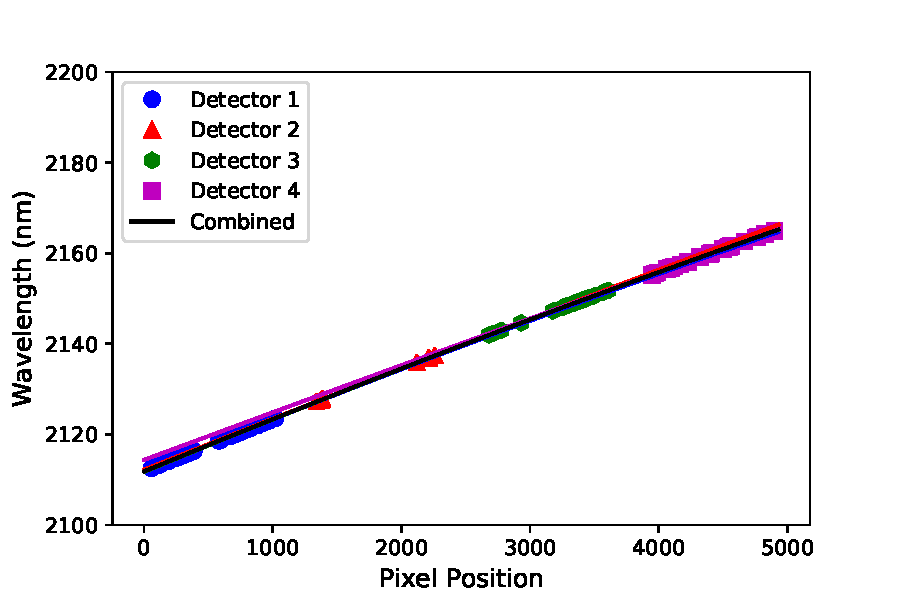
\includegraphics[width=0.75\linewidth]{./figures/appendix/combined_wav_fit}
    \caption[Multi-detector fit and difference to individual fits.]{Pixel-wavelength calibration points for each detector are given by the different markers. The quadratic fit of each individual detector is given with the same corresponding colour. A combined quadratic fit, using fixed detector gaps is shown in black.}
    \label{fig:multidectorfit}
\end{figure}


\begin{figure}
    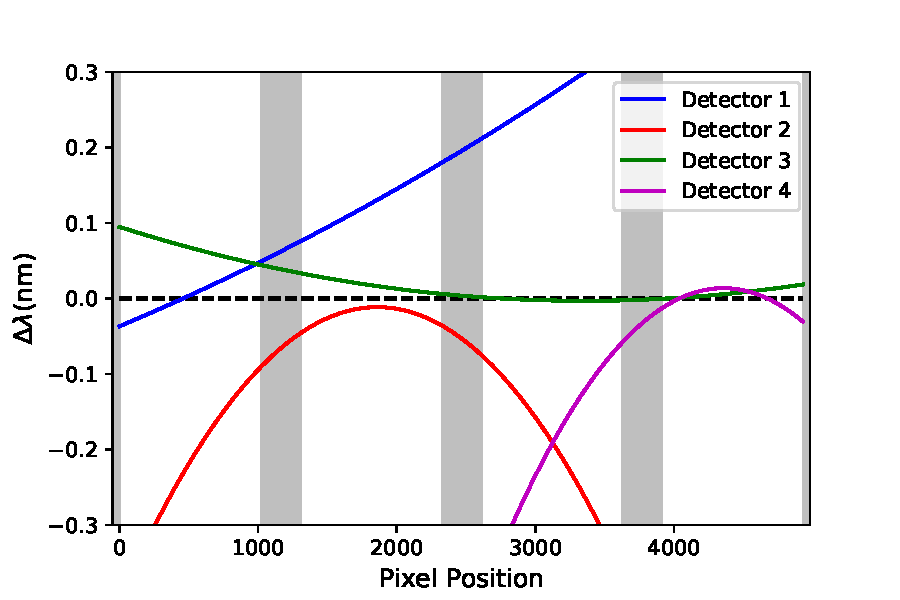
\includegraphics[width=0.75\linewidth]{./figures/appendix/difference_combined_wav_fit}
    \caption[Difference of multi-detector combined fit to the individual calibration mappings.]{Wavelength difference of individual quadratic fits to the quadratic fit combined all four detectors and fixed gaps.}
    \label{fig:multidectorfitdiff}
\end{figure}

The combined fit is made by first assigning each horizontal pixel of each detector the position between 0 and 4095 in pixel coordinates of the {CRIRES} detectors.
A transformation is made into a psudo-physical pixel coordinates from the left edge of the first detector by including the gaps between the detectors (in pixels).
The parameters \(gap_{1}\), \(gap_{2}\), \(gap_{3}\) are the 3 gaps between neighbouring detectors gaps and are defined in pixel space as follows:
\[
gap =\begin{cases}
0,                       & ~~~~0=<pxl<1024\\
gap_1,                    & 1024=<pxl<2048\\
gap_1 + gap_2,             & 2048=<pxl<3072\\
gap_1 + gap_2 + gap_3,      & 3072=<pxl<4096
\end{cases}
\]

The pixel widths of these gaps can be fixed to known values (e.g.\ 282, 278, and 275 pixels~\citep{brogi_rotation_2016}) or allowed to vary and included in the fitting process.


\subsection{Comparing variable gaps}

\begin{figure}
    \centering
    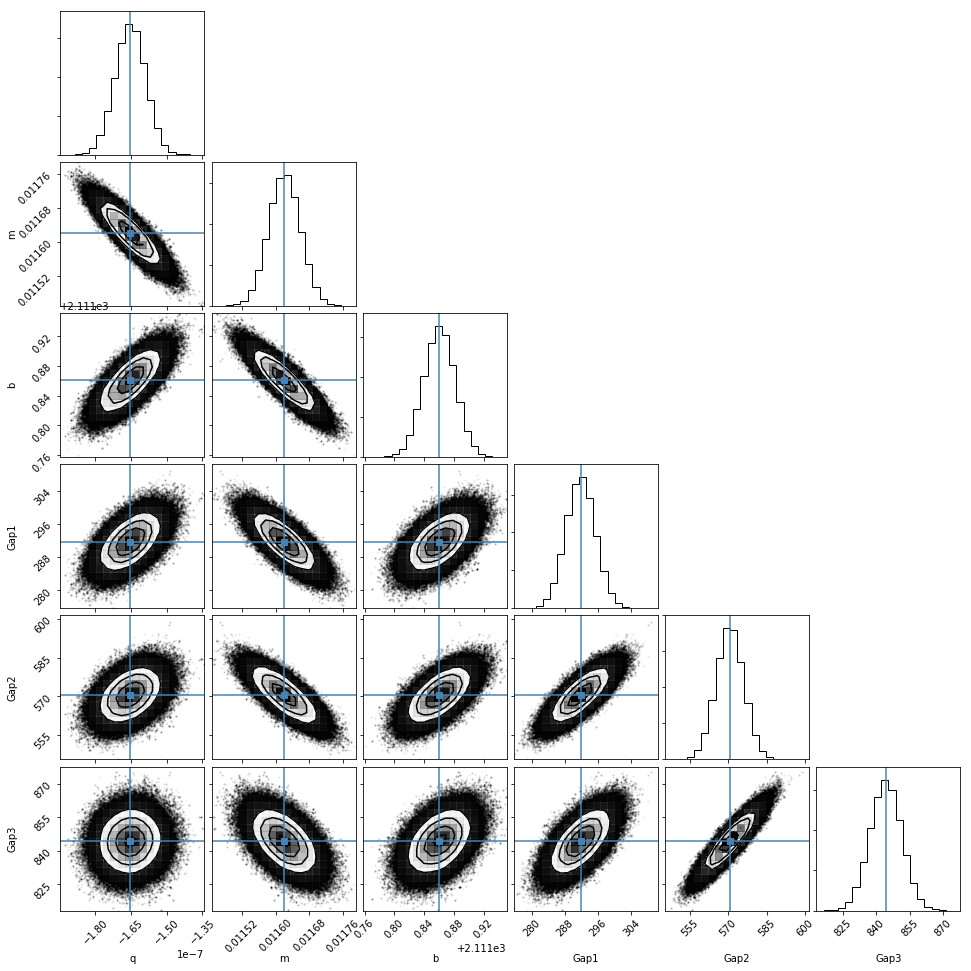
\includegraphics[width=0.5\linewidth]{./figures/appendix/multidetecot_param_fit}
    \caption[Multi-detector parameter correlations.]{Corner plot of emcee combined fitting.
    The elliptical point clouds indicate there are correlations between parameters.}
    \label{fig:multidetecotparamfit}
\end{figure}

This example does not include the height on the detectors the spectrum falls or any skewness of the spectrum to pixel rows or any miss-alignment between the detectors. All which could have some affect on a global wavelength calibration.

\cref{tab:example_calibration_parametres} shows the fit parameters obtained as well as some fit statistics for quadratic and cubic fitting, comparing the full combined fit with fixed or variable gaps. 

\cref{fig:quadcornerplots} also show the distribution of the fit parameters for the quadratic fit with fixed (left) and variable gaps (right) obtained using the \textit{emcee} python package\footnote\href{http://dfm.io/emcee/current/}{http://dfm.io/emcee/current/}}, which performs a Markov chain Monte Carlo simulation.
The cloud of points reveal the correlations between different parameters.
For instance the narrow diagonals indicate a strong correlation between the parameters given on the axis.
There are strong correlations between the quadratic parameters, {q, m, b} with $m$ being negatively correlated to all other parameters.
It also shows strong positive correlations between the variable detector gaps.

They plot on the left with fix detector gaps, is almost identical to the top 3 rows of the figure on the right.


\begin{table}
    \small
    \caption[Example of multi-detector fitting parameters and correlation.]{Example of multi-detector fitting parameters obtained for the second observation of HD\,30501 under different scenarios.
        Second and third order polynomials are indicated by \(2^\circ\) and \(3^\circ\) respectively.}
    \begin{tabular}{lcccccccccccc}
        \toprule
        & \multicolumn{2}{c}{Fixed Gaps} & \multicolumn{2}{c}{Variable Gaps} \\
        \midrule
        Order & \nth{2} & \nth{3} & \nth{2} & \nth{3} \\
        a3 (u) & - & $(-2\pm 3) \times 10^{-12}$ & - & $(-2 \pm 1)\times 10^{-12}$ \\
        a2 (q) & $(-1.77 \pm 0.03) \times 10^{-7}$ & $(-1.6 \pm 0.2)\times 10^{-7}$ & $(-1.65 \pm 0.06) \times 10^{-7}$ & $(-1.47 \pm 0.07)\times 10^{-7}$ \\
        a1 (m) & $0.01170 \pm 0.00002$ & $0.01167 \pm 0.00005$ & $0.01162149 \pm 0.00004$ & $0.01160 \pm 0.00001$  \\
        a0 (b) & $2111.83 \pm 0.01$ & $2111.84 \pm 0.02$ & $2111.86 \pm 0.02$ & $2111.87 \pm 0.01$ \\
        \(gap_{1}\) & 283 & 283 & $291.7 \pm 3.5$ & $291.2 \pm 0.9$ \\
        \(gap_{2}\) & 561 & 561 & $570.5 \pm 5.4$ & $567.9 \pm 1.7$ \\
        \(gap_{3}\) & 836 & 836 & $844.2 \pm 7.1$ & $841.3 \pm 2.1$ \\
        \textchisquared{} & 11.2 & 10.7 & 4.6 & 4.2 \\
        \textchisquaredreduced{} & 0.156 & 0.151 & 0.066 & 0.061 \\
        {BIC} & -129.3 & -128.6 & -184.1 & -186.7 \\
        \bottomrule
    \end{tabular}\label{tab:example_calibration_parameters}
\end{table}

\begin{figure}
    \centering
    \begin{tabular}{c c}
    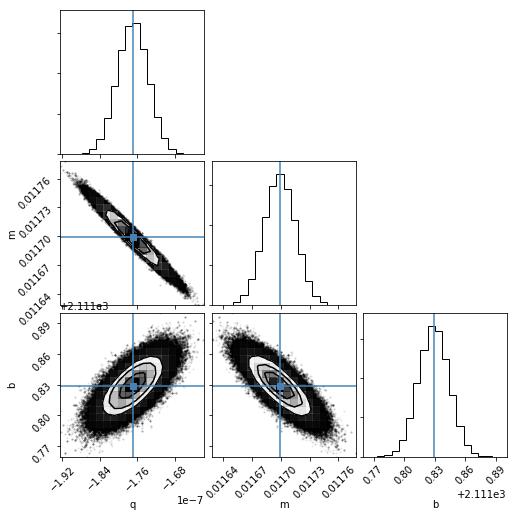
\includegraphics[width=0.7\linewidth]{figures/appendix/fixed_quad_corner} & 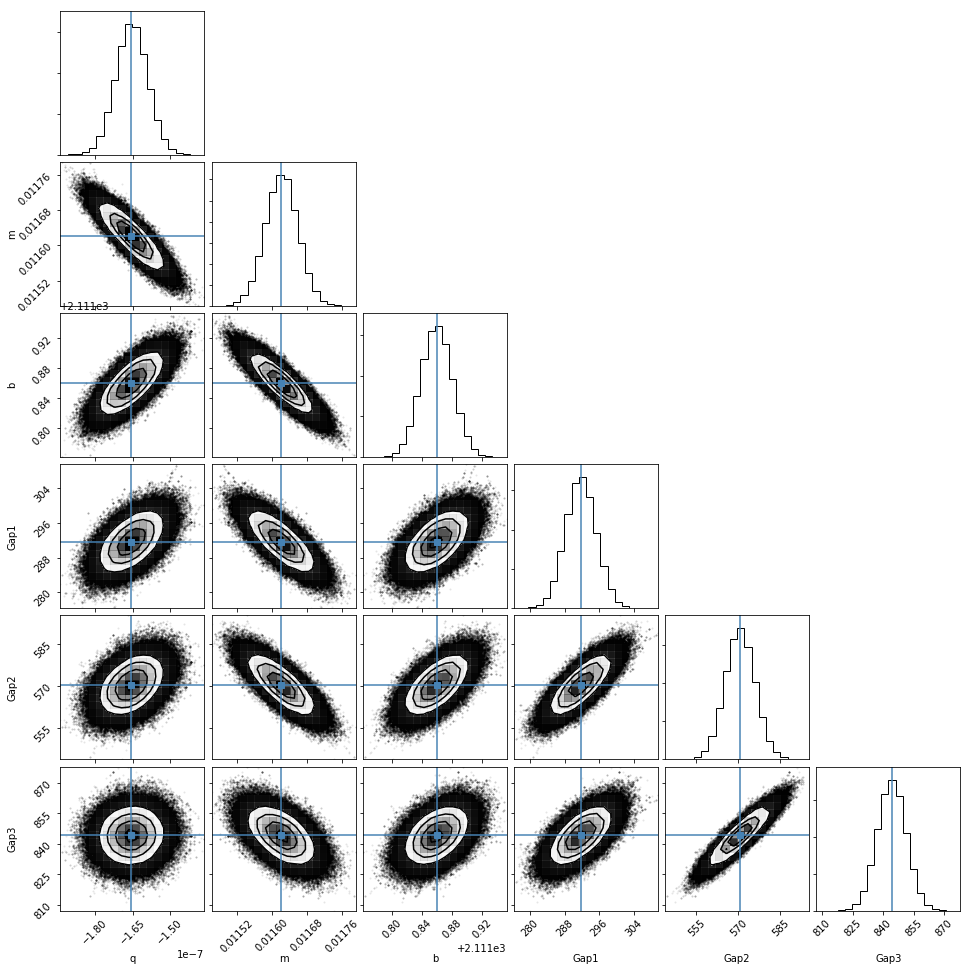
\includegraphics[width=0.7\linewidth]{figures/appendix/variable_quad_corner} \\
    \end{tabular}
    \caption{}
    \label{fig:quadcornerplots}
\end{figure}

This is just a simple representation of the idea, it has not been used in this thesis for wavelength calibration

\todo{reread and fix up still}